\section{JaCaMo}

JaCaMo è un framework per la programmazione orientata agli agenti che combina tre tecnologie già affermate e sviluppate da diversi anni. Come ogni MAS, JaCamo fornisce agli sviluppatori e ai designer tre astrazioni principali:
\begin{itemize}
    \item Agenti: Le entità autonome che compongono il sistema. Sono in grado di comunicare e possono essere intelligenti, dinamici, e situati;
    \item Società: Rappresenta un gruppo di entità il cui comportamento emerge dall'interazione tra i singoli elementi;
    \item Ambiente: Il "contenitore" in cui gli agenti sono immersi e con il quale questi ultimi possono interagire apportandogli modifiche. La caratteristica degli agenti di essere situati nell'ambiente in cui si trovano permette loro di percepire e produrre cambiamenti su di esso.
\end{itemize}

Un sistema multi-agente JaCaMo o, equivalentemente, un sistema software programmato con JaCaMo è definito da un'organizzazione Moise di agenti BDI autonomi basati su concetti come ruoli, gruppi, missione e schemi, implementati tramite Jason, che lavorano in ambienti condivisi distribuiti basati su artefatti, programmati in CArtAgO.

\medskip

Ognuna delle tre tecnologie indipendenti che compongono il framework ha il proprio set di astrazioni, modelli di programmazione e meta-modelli di riferimento; per questo motivo in JaCaMo è stato realizzato un meta-modello globale avente l'obiettivo di definire dipendenze, connessioni, mapping concettuali e sinergie tra le differenti astrazioni rese disponibili da ogni livello.\cite{BOISSIER2013747}

\begin{figure}[H]
\centering
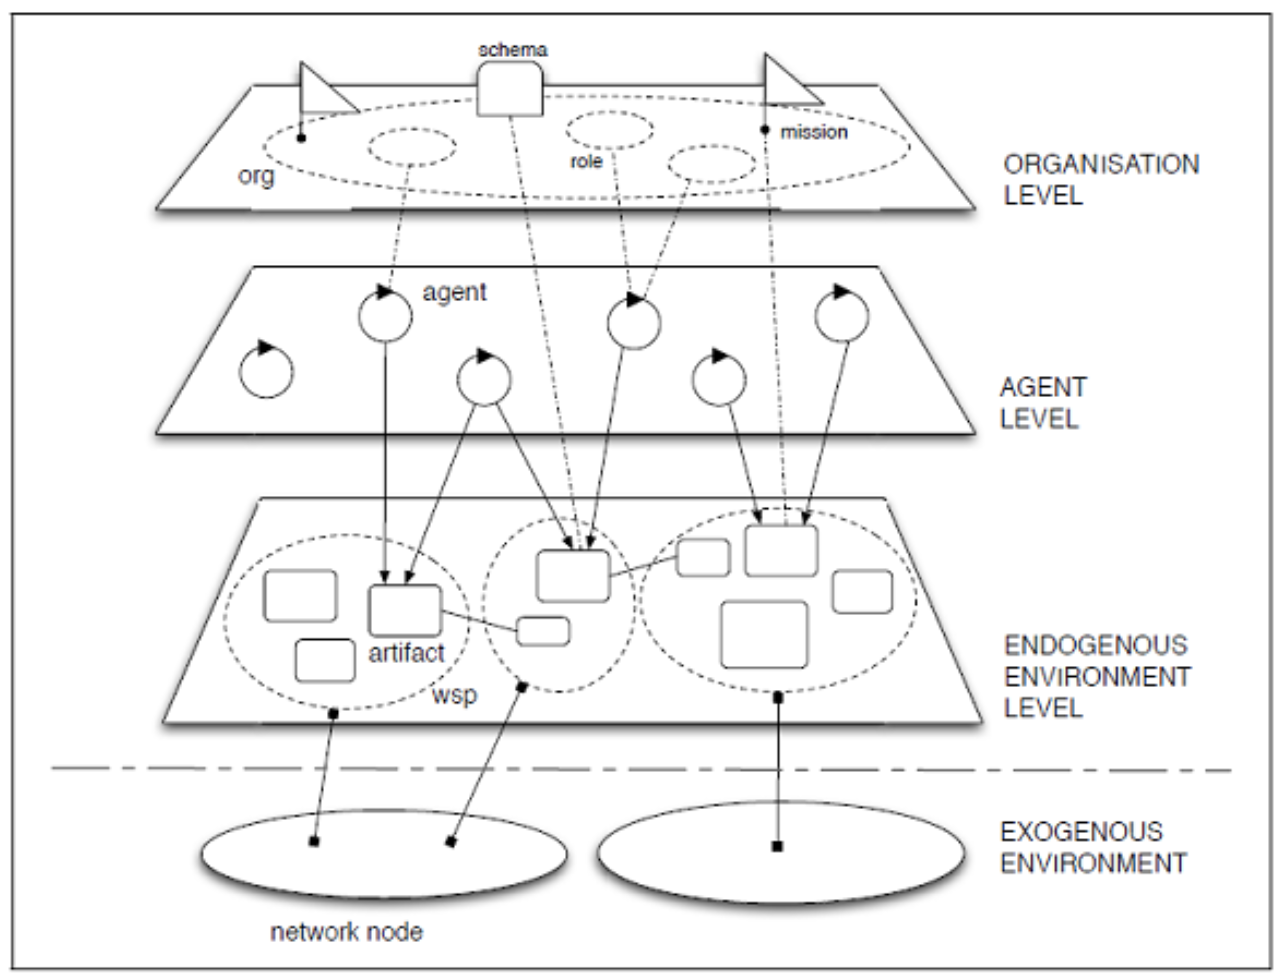
\includegraphics[width=\textwidth]{figures/JaCaMo_levels.png}
\caption{Livelli che compongono il framework JaCaMo\cite{BOISSIER2013747}}
\label{livelli_jacamo}
\end{figure}

\subsection{Jason} \label{jason}

Jason è un interprete di AgentSpeak che implementa la semantica operazionale del linguaggio e fornisce una piattaforma di sviluppo per multi-agent systems con molte funzionalità user-customisable.

\medskip

Le astrazioni appartenenti agli agenti, correlate al meta-modello Jason, sono principalmente ispirate all'architettura BDI sulla quale Jason è radicato. Quindi un agente è un'entità composta da un insieme di "beliefs" che rappresenta lo stato corrente e la conoscenza dell'agente sull'ambiente in cui si trova; una serie di "goals", che corrispondono a compiti che l'agente deve eseguire / ottenere e una serie di "plans", ossia azioni (external action or internal action) innescate da eventi, che gli agenti possono comporre, istanziare ed eseguire dinamicamente per compiere i "goals".\cite{jason-book}

\begin{figure}[H]
\centering
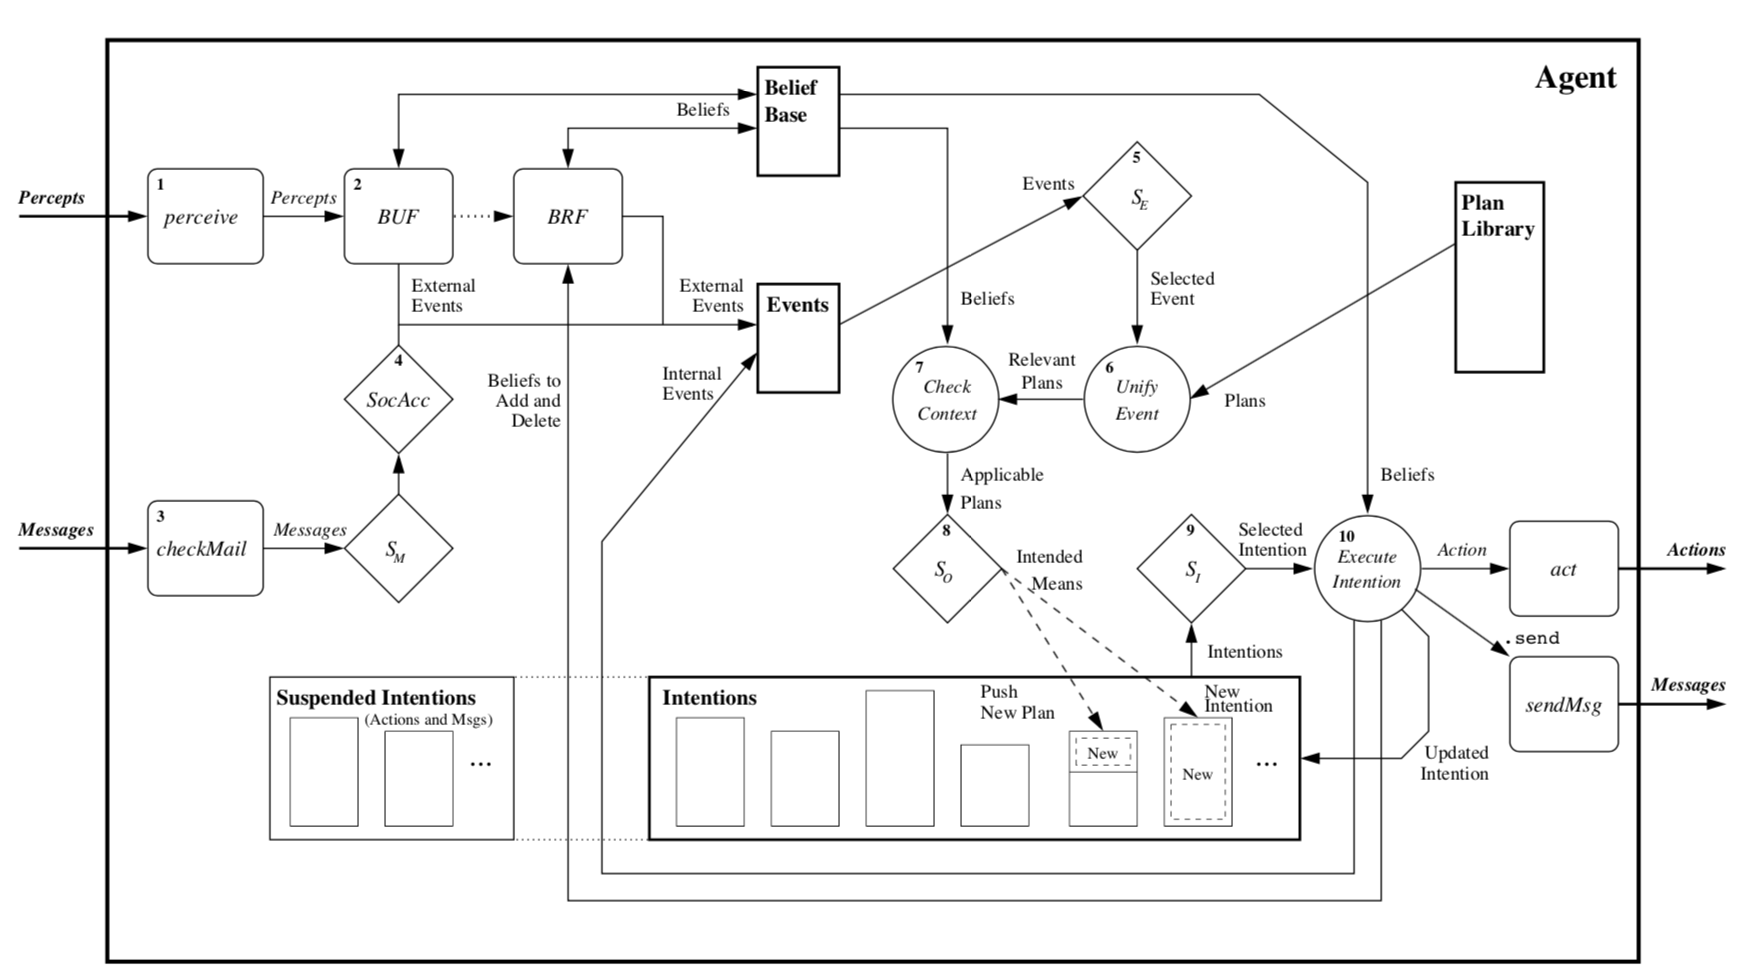
\includegraphics[width=\textwidth]{figures/Agent_BDI_Lifecycle.png}
\caption{Architettura BDI di un agente\cite{jason-book}}
\end{figure}

Durante l'analisi delle astrazioni disponibili su Jason è risultato particolarmente utile, al fine di integrazione con la Game Engine, il concetto di "beliefs". 

\medskip

La Belief Base, raffigurata nell'immagine soprastante, è il contenitore della conoscenza dell'agente che viene in parte modificata dalle percezioni esterne che l'agente riceve dall'ambiente. Tali percezioni sono facilmente riconducibili alle percezioni / eventi che un GameObject può ricevere durante la sua permanenza nella scena (spiegato nella sezione \ref{ambiente_unity}), come ad esempio la notifica di una collisione con un secondo GameObject in scena. 

\medskip

Questo concetto ha portato alla decisione di utilizzare il belief come strumento di "notifica" delle percezioni ricevute dal GameObject su Unity, con lo scopo di integrare i due sistemi senza effettuare modifiche su concetti e astrazioni di MAS e Game Engine.

\subsection{CArtAgo}
Ciascuna istanza dell'ambiente CArtAgO\footnote{Common ARTifact infrastructure for AGents Open environments} è composta da una o più entità workspace. Ogni workspace è formato da un insieme di artefatti, che forniscono un insieme di operazioni e proprietà osservabili, definendo anche l'interfaccia di utilizzo degli artefatti. L'esecuzione dell'operazione potrebbe generare aggiornamenti delle proprietà osservabili e degli eventi osservabili specifici. L'ultima entità relativa all'ambiente è il “manual”, un'entità utilizzata per descrivere le funzionalità fornite da un artefatto.
Cartago è basato sul meta-modello A\&A (Agents \& Artifacts) gli agenti come delle entità computazionali compiono qualche tipo di attività che mira a uno scopo e, gli artefatti come risorse e strumenti costruiti dinamicamente, sono usati e manipolati dagli agenti per supportare/realizzare le loro attività.\cite{cartago}

\smallskip

\paragraph{Artefatto}
L'artefatto è un'entità reattiva, non autonoma, stateful, riutilizzabile, controllabile ed osservabile. Modella strumenti, risorse e porzioni di ambiente agendo da strumento mediatore di azioni e interazioni sociali tra partecipanti individuali e lo stesso ambiente.\cite{Omicini2008} 

\begin{figure}[H]
\centering
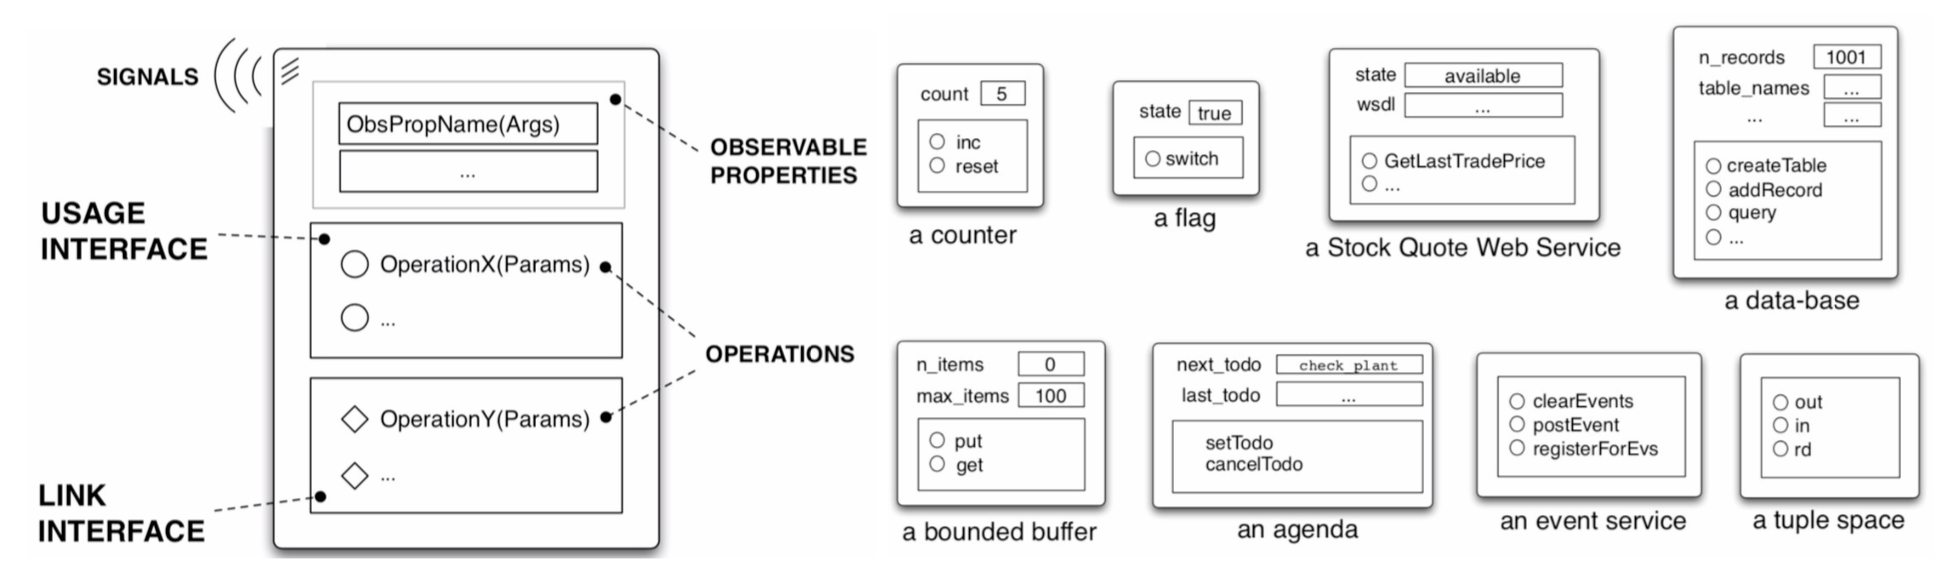
\includegraphics[width=\linewidth]{figures/Artifact_structure_example.png}
\caption{Struttura artefatto con relativi esempi}
\end{figure}

Durante l'analisi delle astrazioni disponibili su CArtAgo sono risultate utili, al fine di integrazione con un Game Engine, i concetti di artefatto, "Observable Properties" e di "Operations". L'immagine sottostante contiene un esempio di interazione e utilizzo tra agente ed artefatto dove viene fatto uso dei concetti precedentemente elencati.

\begin{figure}[H]
\centering
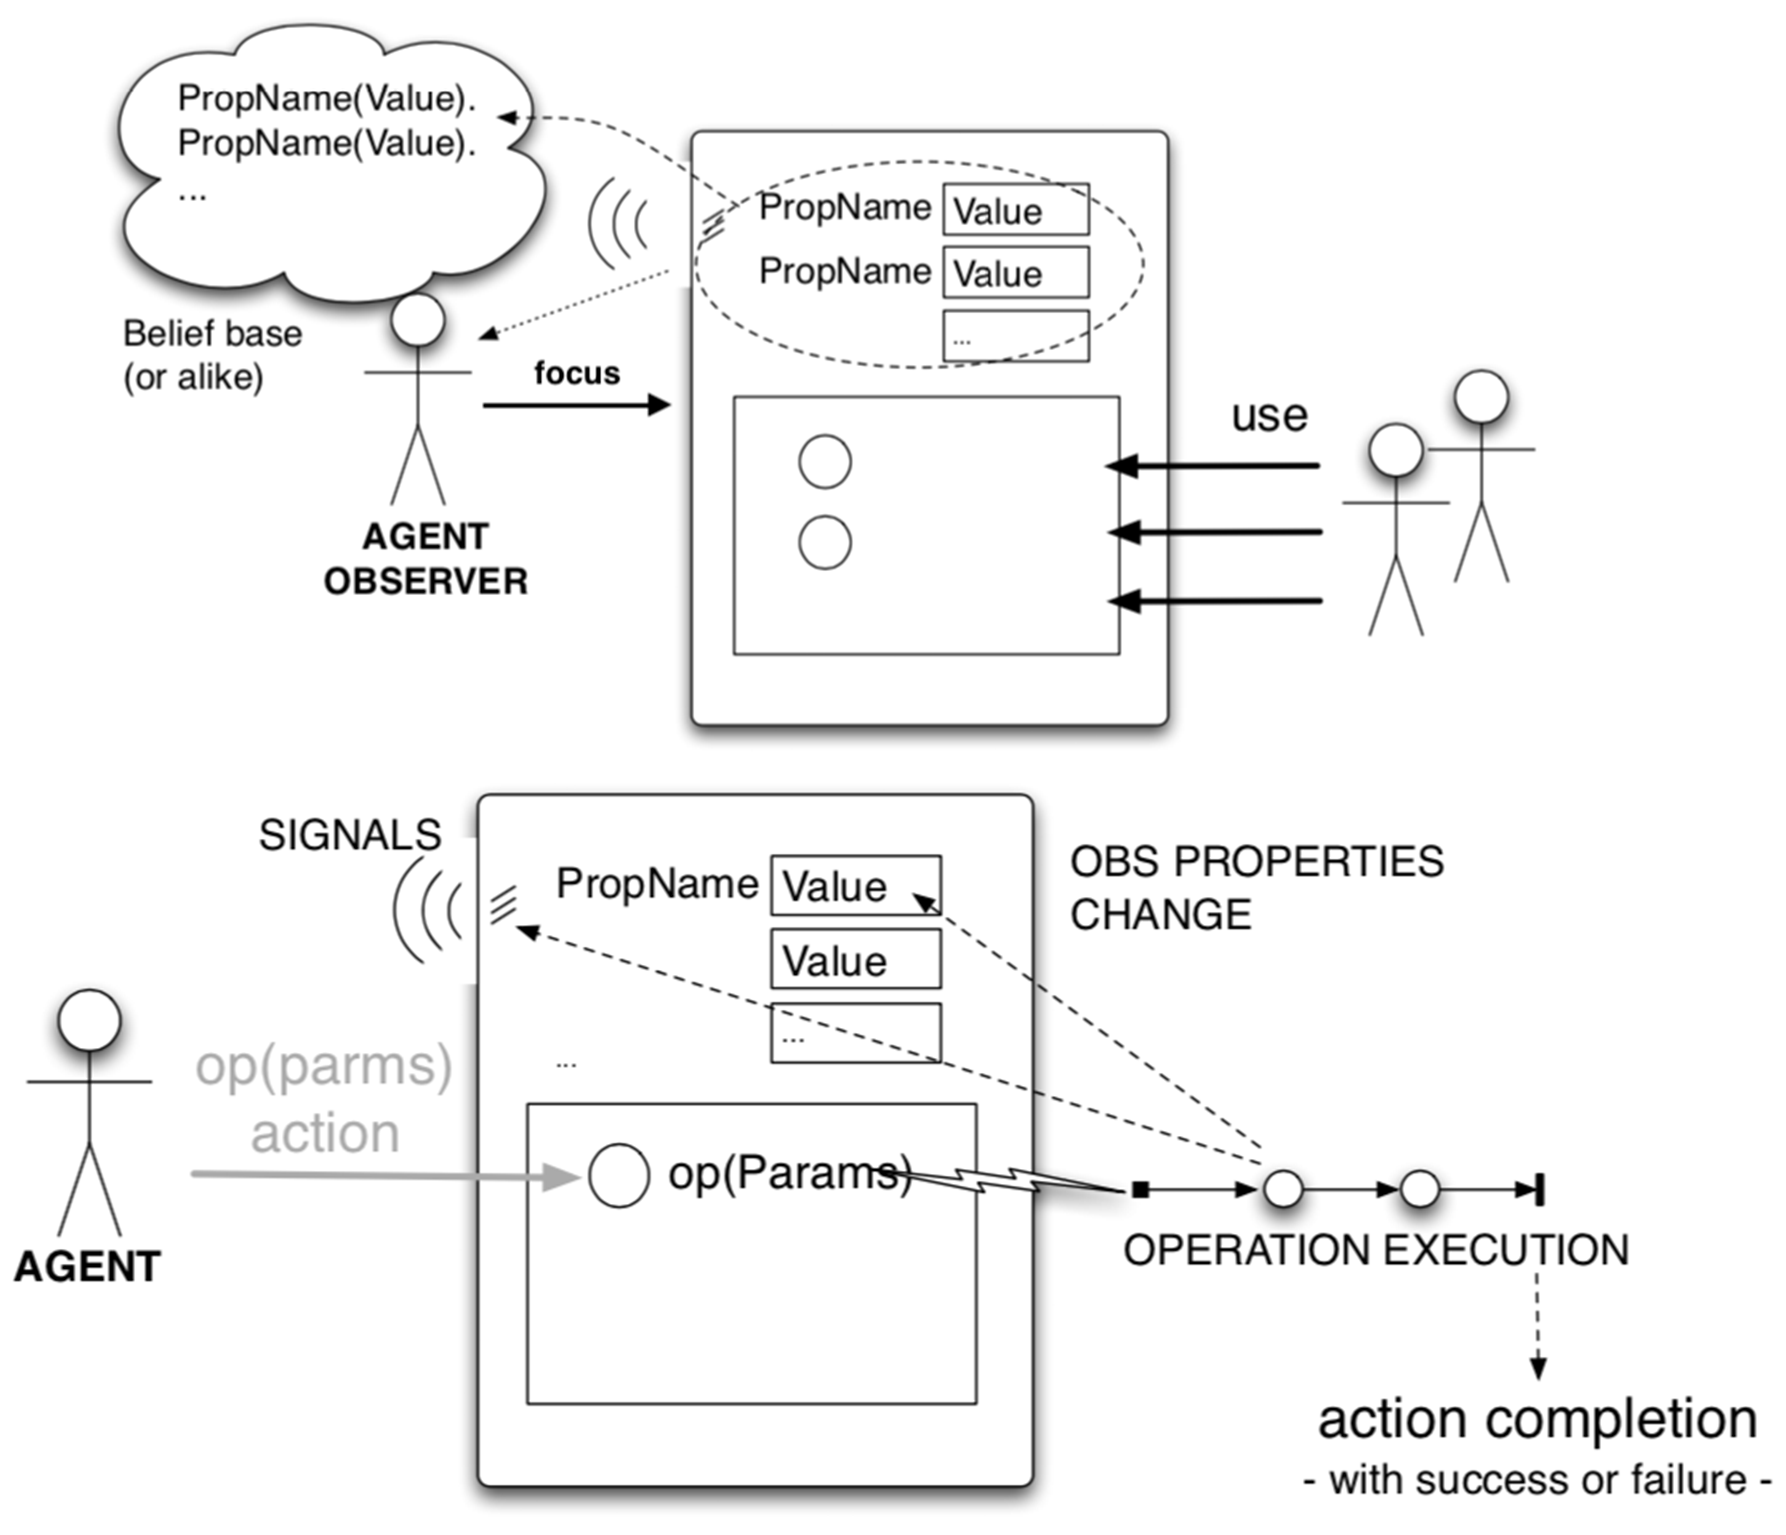
\includegraphics[width=\linewidth]{figures/Artifact_use.png}
\caption{Interazione ed utilizzo tra agente ed artefatto}
\end{figure}

La definizione di artefatto ha contribuito a definire la principale modalità di integrazione tra MAS e Game Engine dato che le sue finalità sono collegabili alle finalità di utilizzo del GameObject su Unity. Entrambi devono rappresentare una porzione di ambiente, risultare uno strumento a disposizione dell'agente per effettuare operazioni/azioni sull'ambiente e "notificare" l'agente in caso di modifiche sulle informazioni contenute. Per questo motivo è stato deciso di effettuare un collegamento univoco tra GameObject e Artefatto con un rapporto di 1:1.

\medskip 

Questa modalità permette quindi ad un agente di utilizzare il proprio artefatto come se fosse il proprio GameObject su Unity e, quindi, di effettuare azioni- utilizzando le "Operations" dell'artefatto- e ricevere informazioni sullo stato del proprio corpo fisico, attraverso le "Observable Properties", senza modificare concetti e astrazioni presenti nel MAS. 

\subsection{Moise}
Moise è un meta-modello organizzativo per MAS basato sulle nozioni di ruoli, gruppi e missioni. Abilita un MAS ad avere specifiche esplicite per la sua organizzazione. Queste specifiche sono usate sia dagli agenti, per ragioni inerenti la loro organizzazione, sia da una piattaforma organizzativa che si assicuri che gli agenti seguano le specifiche.

\medskip

Moise consente di definire una gerarchia di ruoli con autorizzazioni e missioni da assegnare agli agenti. Questo permette, ai sistemi con un'organizzazione forte, di guadagnare proprietà di apertura (essenzialmente, la proprietà di lavorare con un numero e una diversità di componenti che non è imposta una volta per tutte) e adattamento.
